\documentclass{llncs}

\usepackage{comment}
\usepackage{graphicx}

%\newcommand{\comment}[1]{{\bf *** #1}}
\newcommand{\lang}{K}

\title{\lang{}: A Wide Spectrum Development Language}
\author{Klaus Havelund and Rahul Kumar}
\institute{
  Jet Propulsion Laboratory\\
  California Institute of Technology\\
  California, USA
}

\begin{document}

\maketitle 

We propose to build a language, named \lang{}, for developing software
systems at a high level of abstraction as well as at a low level of
implementation. The language should allow a user to first specify a
system at a high level, and then at later stages refine this
specification into a detailed program, all within the same language.
Checks and balances should be performed to ensure that the detailed
refinement implements the abstraction. Such checks can be performed
statically as well as dynamically. That is, \lang{} language should be
supported by analysis tools of various kinds, including static
analysis, verification, and dynamic analysis (testing/runtime
verification). In general, \lang{} should be a vehicle and platform
for experimenting with various ideas related to developing correct
programs fast.


\section{Background}
This work is inspired by various sources. One major influence is the
set of formal specification languages such as VDM/VDM++, Z etc. These
languages contain features such as functional programming/modeling
with higher order functions; algebraic data types; pattern matching;
object oriented programming/modeling with variables; assignment
statements; loops etc; design by contract with pre/post conditions and
class invariants; and general higher order predicate logic for writing
Boolean expressions. VDM++ never became mainstream, although it was
one of the main formal methods before theorem proving and model
checking became popular.  One reason for not lasting was probably in
part that it was a specification language, and not a programming
language, and in part, because there was no serious tool
support. Proofs, if any, would have to be carried out manually.  Our
objective is to turn this around and define a wide-spectrum {\bf
  programming} language inspired by the same ideas, and use the latest
results in automated verification as basis for tools.

A second inspiration is our current work to provide a textual
language, named K, for SysML, to be used to design the proposed
Europa Clipper mission. SysML is a graphical language for creating
models of systems (in contrast to models of software, as is the target
of UML). SysML contains selected elements of UML but also extends
it. SysML engineers recognize that there is a need for a textual
modeling language in addition to the graphical, such that ideally one
can create/view a model in either format, depending on taste and
situation. The main challenge here is to make the relational view
adopted in SysML (there are only atomic objects and relations between
them) co-exist with the data type view present in most other
languages, where there are data types such as collections (sets, lists
and maps). This challenge corresponds to combining traditional
programming with database/logic programming.

\begin{comment}
As it turns out, the SysML team at JPL has asked for a textual
language very much along the lines of VDM and Z. This in itself is
interesting: that the SysML/UML community sees a need for the kind of
languages that formal methods came up with decades ago. 
\end{comment}

A third inspiration is the current trend in programming language
design, which seems to move towards the combination of object oriented
and functional programming with high-level concepts such as
collections (sets, lists, and maps), iterators, and generally all the
concepts from VDM++ except general predicate logic in Boolean
expressions. 

Finally, we also draw inspiration from related work done by Mihai
Florian and Gerard Holzmann at JPL. Their work laid less emphasis on
high level programming but more on specification constructs with a
verification environment surrounding them.

Figure~\ref{fig:influences} graphically depicts the various influences
on \lang{}. 

\begin{figure}
  \label{fig:influences}
  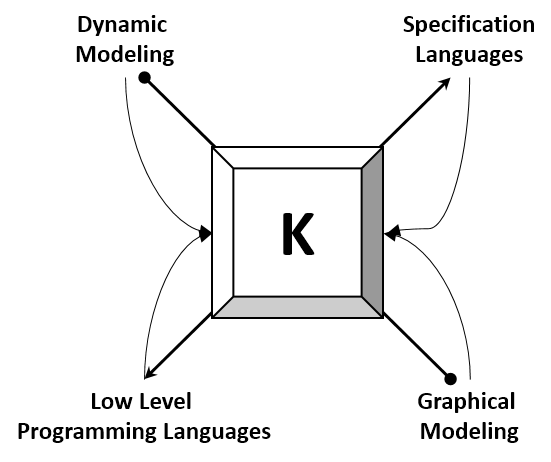
\includegraphics[scale=0.75]{influences.png}
  \centering
  \caption{Influences on \lang{}}
\end{figure}

\begin{comment}
There has also been programming languages in the past, such as SETL,
which focused on set theory, also an inspiration.

Finally, the work of Mihai Florian guided by Gerard Holzmann was in
this line, although there was less emphasis on high-level
programming. The focus was exactly to design a programming language
with specification constructs, and with a verification environment
around it. Similar attempts are made with languages such as Spec\# and
Dafny from MSR. One might also mention the work on SPOT here at JPL,
and perhaps even unite with that work.

All in all, attempts have been made are being made in this
direction. Yet, it is an interesting avenue of research that we should
take on. 
\end{comment}

\section{What}

\begin{comment}
We would consider the current K language (textual version of SysML) as
our starting point, or we simply consider the K language as the
language, and as a group collectively focus on supporting the Europa
project, the latter probably being more practical.  The Europa project
wants this language, they claim they rely on it to {\em ``clean up the
  SysML mess''}.  There is a certain pressure to get this right.
\end{comment}

\lang{} is intended to be a wide-spectrum language that supports
various scenario such as programming, modeling, specifcation, or a
combination of the same. We now list the features of the language that
we believe will make it possible for \lang{} to be a wide-spectrum
language:

\begin{comment}
The language should be one that each of us would want to program our
systems in. Hence it should be as fast as C when staying in the low
level fragment.  We would discuss which fundamental paradigm the
language should built on: object-oriented? functional?,
logic-programming?, data-base technology? (currently K has relations,
which resemble relational databases). We would discuss whether it will
make sense to let the language allow abstract specification as well as
low-level C-like programming. Is it possible to merge these concepts?
Ocaml is claimed to be as fast as C and combines the two
levels. Garbage collection could get in the way.
\end{comment}

\begin{itemize}
  \item \textbf{Programming constructs}:
    \begin{itemize}
      \item object-oriented features, including classes and objects,
        variables, assignment (side effects), sequential composition,
        loops, etc, standard stuff.
      \item functional programing, including functions as values,
        algebraic data types, pattern matching.
      \item Built-in collections such as sets, lists and maps,
        including iterator constructs over such.  Can be libraries,
        but special syntax for sets, lists and maps is attractive.
      \item Should be garbage-collected for ease of
        programming. However, this is a challenge in the context of
        embedded systems. Will require research.
      \item Concurrency constructs inspired by modern actor frameworks
        (message passing).
      \item Support for extending the language and define DSLs. This
        includes serious reflection capabilities, such that a program
        can examine itself. For example, a coding standard can just be
        a library one imports.
      \item The work on the relational view in SysML opens the
        question whether it would be useful with a graph-model as part
        of the language: relations, logic-programming.
    \end{itemize}
 
  \item \textbf{Specification constructs}:
    \begin{itemize}
      \item pre/post conditions and invariant specifications for functions
      \item class invariants.
      \item temporal logic-like specifications over execution traces
        (can be rule-based, regular expressions, etc.).
      \item General predicate logic for writing Boolean expressions.
      \item refinement: the language should support the notion of
        refinement within the language: for example that a class
        implements another class, resulting in a proof-obligation to
        show that it is true. That can be checked statically or
        dynamically during execution.
    \end{itemize}
\end{itemize}

Apart from the language itself, we envision the development of a suite
of tools that enable the scenarios listed above. They are as follows:

\begin{description}

  \item [Compiler] for producing executable code. Initially, for
    prototyping, this may be to a high-level language, such as Scala
    or C, and later to low-level machine code such using the LLVM
    framework.

  \item [Verifiers] including static analysis, model checking, theorem
    proving (Dafny style), etc.
    
  \item [Tester] including runtime verification, test-case generation,
    and unit-testing. Testing would include machine learning: learning
    specifications from execution traces, which can later be turned
    around to monitors, be visualized, or even perhaps proven against
    the code using some form of theorem proving.
    
  \item [Visualizer] static (of program structure) as well as dynamic
    (of execution traces). The visualization can be interactive, such
    that code can also be generated from graphics.  It is important,
    however, that the code is the main representation form, which can
    be visualized.

\end{description}

\section{How}

We propose the development of the language in three primary stages that
are described below:

\begin{description}

\item [Language Design] stage where the language syntax, constructs,
  and features are developed to maturity. We plan on using existing
  tools such as ANTLR for specifying the grammar and creating a
  functional parser.

\item [Language Development] stage where the language is used to
  develop models, programs, and specifications. These may include but
  are not limited to the Europa Clipper mission models and
  specifications. Any feedback from language users would also be
  reviewed and integrated back into the language.

\item [Tool Development] stage where we develop the tools listed
  above. Again, we plan on using some existing technologies such as
  LLVM, Scala, ANTLR etc.

\end{description}

\section{100 Week Target}

A language that includes the grammar along with a toolchain that
supports parsing, analyzing, compiling, and executing programs
produced in \lang{}.

\end{document}
